\documentclass{beamer}
\mode<presentation>
\usetheme{CambridgeUS}
% \usecolortheme{crane}
\usefonttheme{serif}
\usepackage{CJKutf8}
\hypersetup{unicode}
\usepackage{bookmark}
\usepackage{bm}
\usepackage{amsmath}
\usepackage{amssymb}
\usepackage{dsfont}
\usepackage{setspace}
\usepackage{tipa}
\usepackage{relsize}
\usepackage{mathrsfs}
\usepackage{calligra}

\definecolor{myred}{HTML}{A30000}

% To ignore the warning of "pdfauthor"
\makeatletter
\def\Hy@WarnOptionDisabled#1{
    \def\next{#1}%
    \def\ignore{pdfauthor}%
    \ifx\next\ignore%
    \else\Hy@Warning{%
        Option `#1' has already been used,\MessageBreak 
        setting the option has no effect%
    }\fi
}

%%%%%% mini AutoBeamer %%%%%%

\def\section#1{
    \framebreak
    \par {            % The style of section title
        \bfseries \color{myred} #1
    }
}
\def\chapter#1{
    \framebreak
    \begin{center}    % The style of chapter page
        \bfseries \Large\color{myred} #1
    \end{center}
    \framebreak
}

%%%%%%%%%%%%%%%%%%%%%%%%%%%%%%

\makeatother

\begin{document}
\begin{CJK}{UTF8}{hei}
    \title{费曼的奇妙观点}
    \author{LC}

    \maketitle

    \begin{frame}[allowframebreaks]
        \maketitle
\chapter{速度 坐标交换}
\section{位移关系}
然后,我们来看一种更为自然的引入方法。\\
在二维的旋转中,在原来$\theta$的旋转后再旋转一个小角度$\Delta\theta$,然后我们考查$x$轴和$y$轴的位移变化。
\begin{figure}
  \centering
  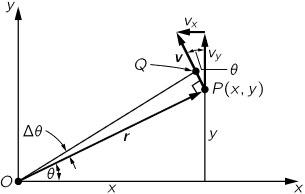
\includegraphics[width=0.3\textwidth]{pic1.png}
  \caption{二维旋转运动学}\label{1}
\end{figure}
\begin{align}
\Delta x & =-PQ \sin\theta=-r\Delta\theta \frac{y}{r}=-y\Delta\theta \\
\Delta y & =+x\Delta\theta
\end{align}
关联的坐标正好交换了!\\
\section{速度关系}
然后我们等式两边同时除以$\Delta t$,根据速度的定义即可得到:
  \begin{equation}
    v_x=-\omega y,\quad  v_y=+\omega x
  \end{equation}
然而,当我们求出速度的大小时,这种奇怪的现象就消失了!
\begin{equation}
  v=\sqrt{v_x^2+v_y^2}=r\omega
\end{equation}
\section{通常推导}
所以在通常的课本上,我们推导时就不会发现这种奇妙的事情。
\begin{align}
  |\Delta \bm{r}|& =r\Delta\varphi \\
  |\Delta \bm{v}|& =\lim_{\Delta t \rightarrow 0} \frac{|\Delta \bm{r}|}{\Delta t}= r \lim_{\Delta t \rightarrow 0}\frac{|\Delta \varphi|}{\Delta t}= \omega r
\end{align}

\chapter{力矩的自然引入}
我们在初中知道,力矩等于力乘上力臂,并且我们通过实验得到了在平衡的杠杆中,力矩是相等的。\\
但是,这未免有些突兀。今天,我们来深入探讨力矩究竟是怎样引入的。\\
\section{二维旋转}
我们知道,功等于力与位移的内积,在一维方向上就是力与位移的大小乘积。但是在二维旋转中,角度是一个重要的量,我们今天将要推导出功与角度的关联量——并将其定义为力矩。\\
将力和微小位移分解到$x$轴和$y$轴上,则力$F$在$x$轴上的分量$F_x$所做的元功为:
\begin{equation}
  \Delta W_x=F_x \cdot \Delta s=F_x \cdot (\Delta x+\Delta y)=F_x \cdot \Delta x
\end{equation}
同理可得,
\begin{equation}
  \Delta W_y = F_y \cdot \Delta y
\end{equation}

将公式(1)(2)代入式子中,可以得到:
\begin{align}
  \Delta W_x&=-yF_x \Delta \theta \\
  \Delta W_y&=xF_y \Delta \theta
\end{align}
则总元功为:
\begin{equation}
  \Delta W=\Delta W_x+\Delta W_y=(xF_y-yF_x)\Delta \theta
\end{equation}
我们将$xF_y-yF_x$定义为力矩,记为$M_{xy}$。\\
我们注意到第一节的奇怪现象:速度关联坐标交换直接影响到了这里力矩的表达式,$x$与$F_y$相乘,$y$与$F_x$相乘。但是这种奇怪的组合事实上涉及一个更广泛的概念。
\section{三维情况}
同样地,在$xOz$和$yOz$平面中,有与$xOy$类似的表达式:
\begin{align}
  M_{xy}&=xF_y-yF_x \\
  M_{xz}&=xF_z-zF_x \\
  M_{yz}&=yF_z-zF_y
\end{align}
这恰好满足叉积的结果,就有:
\begin{equation}
  \bm{M}=\left|
      \begin{array}{ccc}
        \bm{i} & \bm{j} & \bm{k} \\
        x & y & z \\
        F_x & F_y & F_z \\
      \end{array}
    \right|=\bm{r}\times\bm{F}
\end{equation}
\begin{figure}
  \centering
  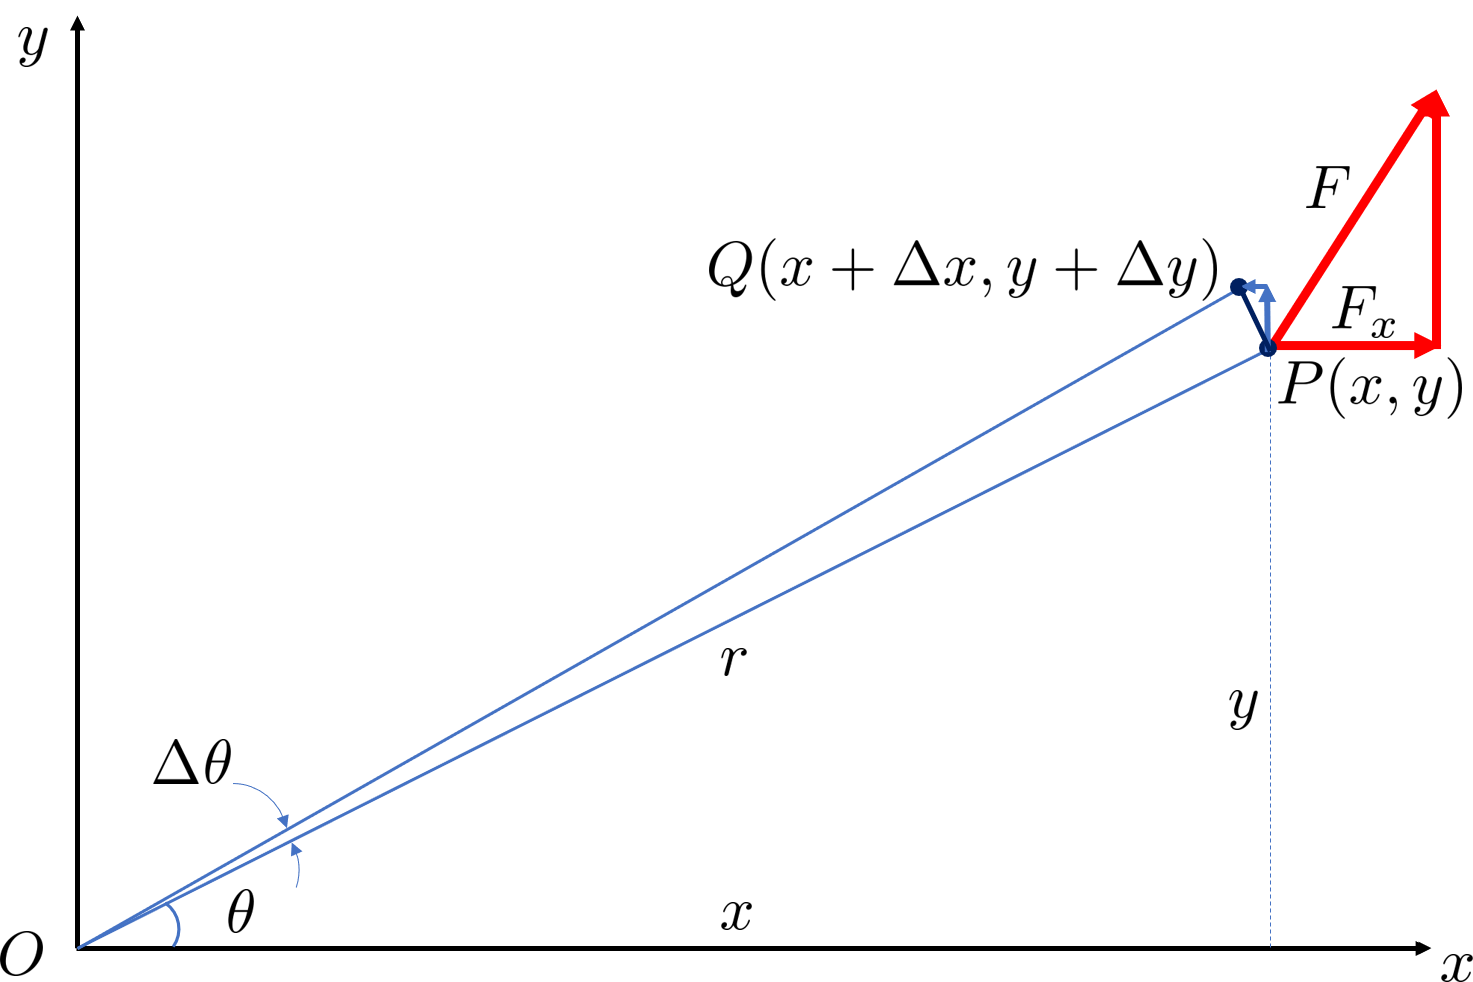
\includegraphics[width=0.5\textwidth]{pic2.png}
  \caption{元功与角度}\label{2}
\end{figure}
这正是课本上的结果!
\section{角动量}
根据牛顿第二定律$F=ma=m\frac{\textrm{d}^2 s}{\textrm{d}t^2}$,我们可将力展开,公式(12)就变成了:
\begin{equation}
  M_xy=xm\frac{\textrm{d}^2 y}{\textrm{d}t^2}-ym\frac{\textrm{d}^2 x}{\textrm{d}t^2}
\end{equation}
奇怪的是,上面的式子是另一个函数的导数:
\begin{equation}
  \frac{\textrm{d}}{\textrm{d}t}\left(xm\frac{\textrm{d}y}{\textrm{d}t}-ym\frac{\textrm{d}x}{\textrm{d}t}\right)
\end{equation}
推导如下:
\begin{align}\nonumber
  \frac{\textrm{d}}{\textrm{d}t}\left(xm\frac{\textrm{d}y}{\textrm{d}t}-ym\frac{\textrm{d}x}{\textrm{d}t}\right)&=xm\frac{\textrm{d}^2 y}{\textrm{d}t^2}+\frac{\textrm{d}x}{\textrm{d}t}m\frac{\textrm{d}y}{\textrm{d}t}-ym\frac{\textrm{d}^2x}{\textrm{d}t^2}-\frac{\textrm{d}y}{\textrm{d}t}m \frac{\textrm{d}x}{\textrm{d}t}\\
  &=xm\frac{\textrm{d}^2 y}{\textrm{d}t^2}-ym\frac{\textrm{d}^2 x}{\textrm{d}t^2}
\end{align}
这正是力矩!
我们将被求导的函数记为角动量,即
\begin{equation}
  L=xm\frac{\textrm{d}y}{\textrm{d}t}-ym\frac{\textrm{d}x}{\textrm{d}t}
\end{equation}
而我们又知道,动量$p=mv=m\frac{\textrm{d}s}{\textrm{d}t}$,所以上式简化为:
\begin{equation}
  L=xp_y-yp_x
\end{equation}
注意比较角动量与力矩形式的相似性。
\section{初中情况}
那这个表达式与初中的力乘上力臂有什么关系呢?
\begin{figure}
  \centering
  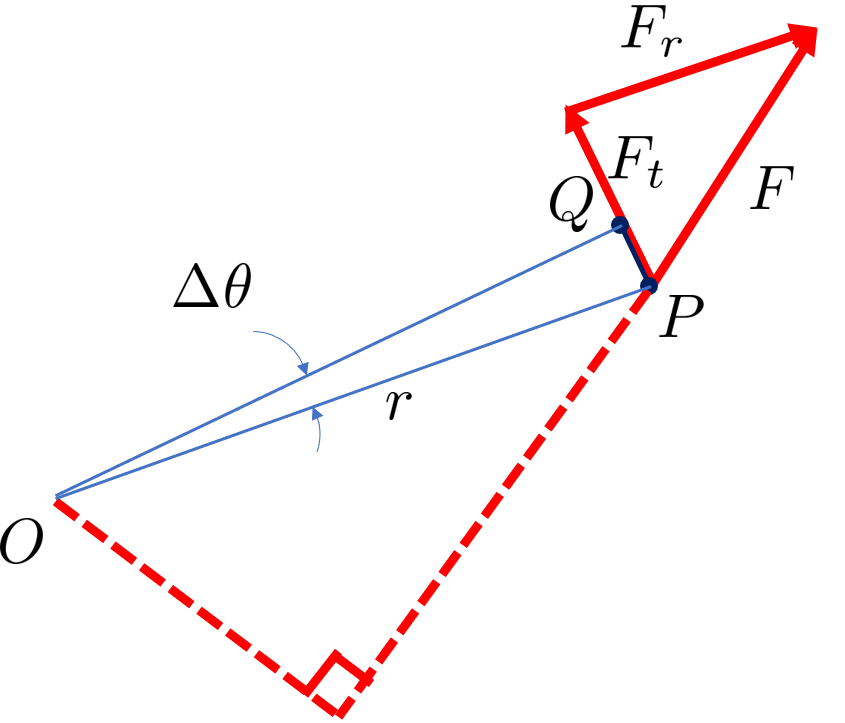
\includegraphics[width=0.5\textwidth]{pic3.png}
  \caption{力矩与角度}\label{3}
\end{figure}
简化图形,将力分解在切向和法向上。在这里元功等于力的切向分量$F_t$与微小位移$\Delta s=r \Delta \theta$的乘积,即
\begin{equation}
  \Delta W=F_t r \Delta \theta
\end{equation}
得到了相同的形式!根据定义,$F_t r$就是力矩了。
有注意到,有两个相似三角形。
\begin{figure}
  \centering
  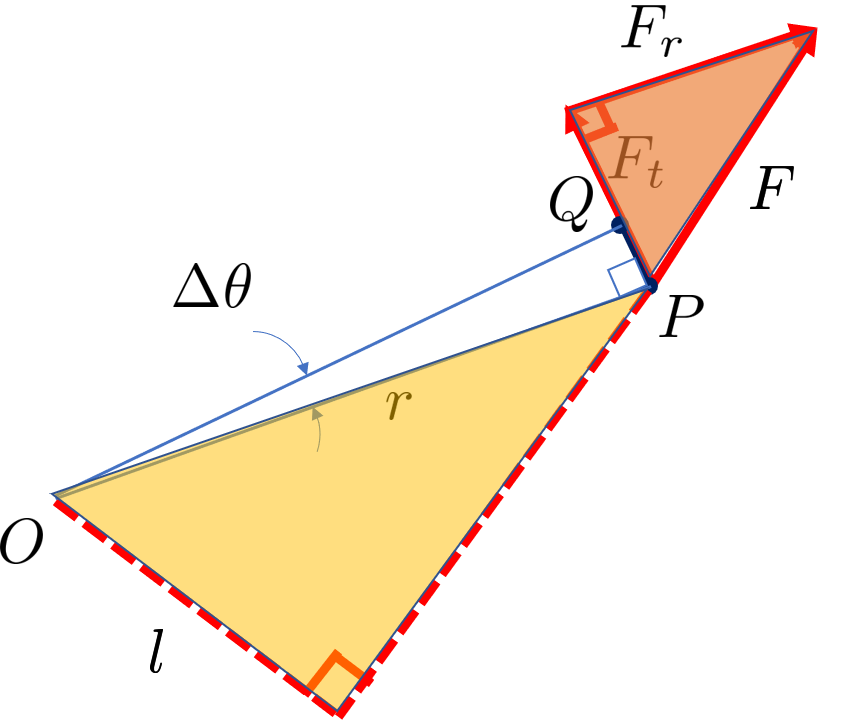
\includegraphics[width=0.5\textwidth]{pic4.png}
  \caption{两个相似三角形}\label{4}
\end{figure}
根据对应边成比例有
\begin{equation}
\frac{F}{r}=\frac{F_t}{l}
\end{equation}
则力矩就变为
\begin{equation}
  M=Fl
\end{equation}
$l$为力臂,这正是初中时候的定义!\\
在上一小节中得到的角动量表达式与力矩形式几乎相同,只是把$F$换成了$p$,则角动量也将有类似的形式
\begin{align}\nonumber
  L &= pl' \\
   \bm{L}&= r\times p
\end{align}
而且下式被称为角动量定理
\begin{equation}
  \bm{M}=\frac{\textrm{d}\bm{L}}{\textrm{d}t}
\end{equation}
\chapter{科里奥利力}
\section{站上传送带}
甲一动不动地站在环形传送带上,随之旋转。乙在地面上静止不动地看着甲。下面从甲的角动量出发,去思考另一种神秘的力——科里奥利力。\\
令甲所在的位置与圆心的距离为$r$,传送带的角速度为$\omega$,甲的质量为$m$,由(4)式得,甲的速度为
\begin{equation}
  v=\omega r
\end{equation}
由(24)式知,甲的角动量为
\begin{equation}
  L=rp=rmv=m\omega r^2
\end{equation}
到目前为止,乙看到传送带在旋转,甲认为传送带是静止的。
\section{迈出一步}
\begin{figure}
  \centering
  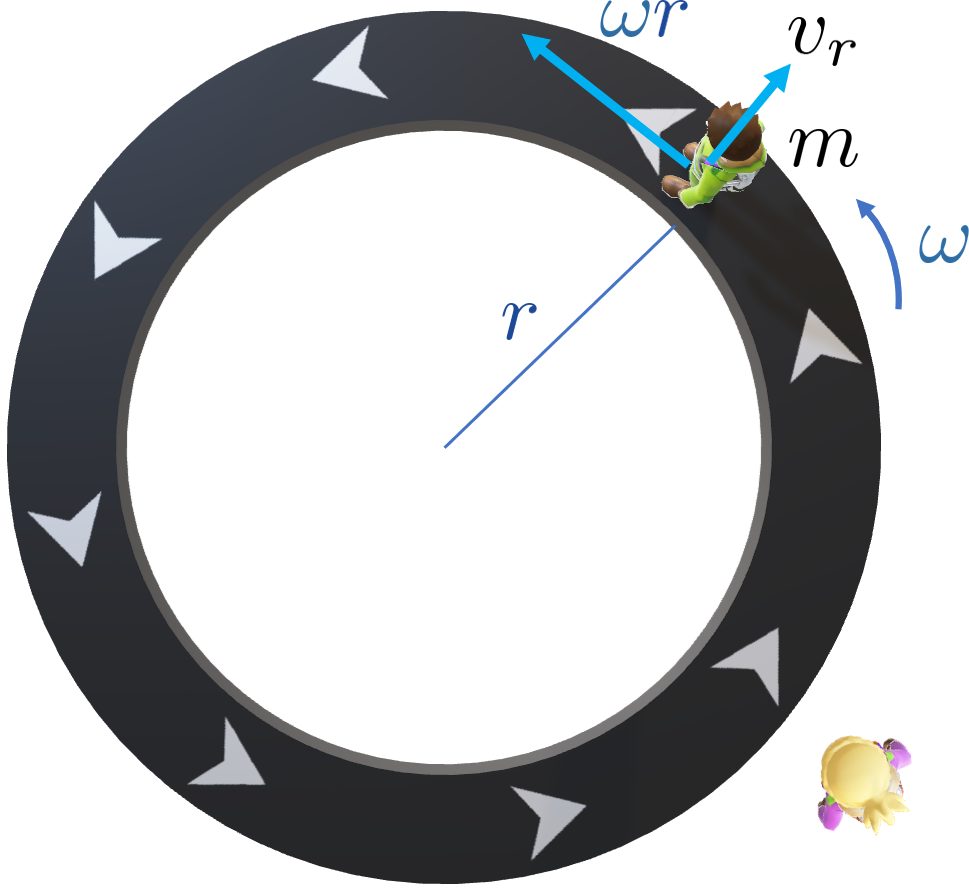
\includegraphics[width=0.5\textwidth]{pic5.png}
  \caption{传送带上的甲与地面上的乙}\label{5}
\end{figure}
接着,甲按耐不住了,相对于传送带,有了一个沿着半径方向的速度$v_r$。但是切向速度是不变的,故在叉乘规则下角动量大小不变,表达式仍为(27)式。\\
不同的是,现在的$r$是一个关于$t$的函数,已非常量。那么为了使角动量改变,一定有一个力矩。假设这个力沿着半径的切向,大小为$F_C$。则
\begin{equation}
  M=F_Cr
\end{equation}
由角动量定理(25)式知,
\begin{equation}
  M=\frac{\textrm{d}L}{\textrm{d}t}=2m\omega r \frac{\textrm{d}r}{\textrm{d}t}
\end{equation}
(28)式和(29)式代表的力矩是同一个力矩,故有
\begin{equation}
  F_C=2m\omega \frac{\textrm{d}r}{\textrm{d}t}=2m\omega v_r
\end{equation}
这个式子可按照叉乘规则改写为
\begin{equation}
  F_C=2m(\bm{v_r}\times \bm{\omega} )
\end{equation}
这个力就被定义为科里奥利力。\\
值得一提的是,当相对速度$\bm{v}$方向不再沿着径向时,上式仍然成立,即
\begin{equation}
  F_C=2m(\bm{v}\times \bm{\omega} )
\end{equation}
\section{直觉}
还是甲相对于传送带的速度沿着径向,站在地上的乙认为甲的运动时两个运动的合成:
\begin{equation}
  \bm{v'}=\bm{v_r}+\bm{\omega}\times \bm{r}
\end{equation}
这是真实速度,故向心力的大小为
\begin{equation}
  F_n=-m\frac{v'^2}{r}=-\frac{mv_r^2}{r}-m\omega^2 r-2m\omega v_r
\end{equation}
而最后一项恰是我们之前定义的科里奥利力!\\
甲能感受到前两项,因为我相对传送带有一个$v_r$的速度,向心力也应该如此,维持甲有这么一个相对速度。第二项是因为甲现有的物理知识能想象得到,如果甲不动的话,这就是甲的向心力。但第三项只看传送带是他是无论如何也不知道的。而第三项是因为我们在不同的参考系下,在这里是由旋转参考系变为乙所在的地面系转换所导致的,所以它和向心力一样,也是一种效果力。
\appendix
\chapter{注释}
\begin{enumerate}
  \item 视频地址(合集):\url{https://www.bilibili.com/video/av40013448/}
  \item LogCreative 个人主页:\url{http://space.bilibili.com/31271993?}
  \item 全文摘自《费曼物理学讲义》(\textit{Feynman Lectures on Physics})第一卷 第18章-第20章,\\在线版网址:
  \begin{itemize}
    \item 第18章:\url{http://www.feynmanlectures.caltech.edu/I_18.html}
    \item 第19章:\url{http://www.feynmanlectures.caltech.edu/I_19.html}
    \item 第20章:\url{http://www.feynmanlectures.caltech.edu/I_19.html}
  \end{itemize}
  \item 视频结尾摘自 Lecture 2 The Relation of Mathematics to Physics|The Characteristic of Physics Law|Richard Feynman\\
  网址:\href{http://www.cornell.edu/video/richard-feynman-messenger-
  lecture-2-relation-mathematics-physics}{视频链接}
  \item 视频中的符号均为加粗,有时代表向量,视情况而定。
  \item 视频与本篇讲义内容或有不妥之处,敬请斧正!
\end{enumerate}
    \end{frame}
\end{CJK}
\end{document}